% !Mode:: "TeX:UTF-8:Main"
% arara: pdflatex
% arara: convert: {density: 96, otheroptions: -dispose previous -delay 20 -loop 1, format: gif}
% xarara: showfile: {format: gif}

% music: https://www.youtube.com/watch?v=dG-62zBnKkQ
\documentclass{article}
\usepackage[utf8]{inputenc} %probably not needed ...
\usepackage[T1]{fontenc}
\usepackage{geometry}
\geometry{papersize={128mm,96mm},margin=0.5cm} %\textwidth=11.8, \textheight=8.6
\usepackage[svgnames,x11names]{xcolor}
\usepackage{tikzducks}
\usetikzlibrary{shapes.geometric}
\pagestyle{empty}
\parindent=0pt
\usepackage{animate}
\usepackage{eso-pic}
\usepackage{xfp}
\tikzstyle{witchstars}=[star, star points=5, star point ratio=2.25, draw,inner sep=1.3pt,anchor=outer point 3]

\makeatletter
\newcommand{\mystar}{%
    \pgfmathsetmacro\xposition{12.4*rnd}
    \pgfmathsetmacro\yposition{8.6*rnd+1}
    \pgfmathsetmacro\starsize{1.8+1.5*rnd}
    \pgfmathsetmacro\starcolor{random(10,75)}
    \ifodd\c@page
    \node[witchstars,fill=yellow!\starcolor!white,inner sep=\starsize pt] at (\xposition,\yposition) {};
    \else
    \node[witchstars,fill=white!\starcolor!yellow,inner sep=\starsize pt] at (\xposition,\yposition) {};
    \fi
    }

\definecolor{finnlandblue}{RGB}{0,53,128}
\tikzset{finnlandflag/.pic={
\begin{scope}[y=0.80pt, x=0.80pt, yscale=-0.03000000, xscale=0.0300000, inner sep=0pt, outer sep=0pt]
% rect98
\path[fill=white,rounded corners=0.0000cm] (0.0000,0.0000) rectangle
  (1800.0000,1100.0000);
\path[fill=finnlandblue,rounded corners=0.0000cm] (0.0000,400.0000) rectangle
  (1800.0000,700.0000);

% rect100
\path[fill=finnlandblue,rounded corners=0.0000cm] (500.0000,0.0000) rectangle
  (800.0000,1100.0000);
  \end{scope}
  }}



\begin{document}
\AddToShipoutPictureBG{%
 \AtPageLowerLeft{%
 
\begin{tikzpicture}[overlay,remember picture]
 \fill[DeepSkyBlue3!50!black] (0,0) rectangle (\paperwidth,\paperheight);
 \pgfmathsetseed{9}
 \foreach \x in {1,2,...,80}{\mystar}
 \end{tikzpicture}}}
\centering
\mbox{}

\medskip\hspace*{0.5cm}%
\begin{tikzpicture}

\begin{scope}
[xshift=313pt-0.5cm,yshift=171pt,y=0.80pt, x=0.80pt, yscale=-0.75000000, xscale=-1.05000000, inner sep=0pt, outer sep=0pt,rotate=-20]
      \path[fill=Silver,draw=LightPink,thick]
        (28.1810,234.4030) .. controls (24.5760,232.5020) and
        (20.1130,233.8830) .. (18.2100,237.4890) .. controls (16.3100,241.0940) and
        (17.6900,245.5590) .. (21.2960,247.4590)
        -- (239.8290,363.9620) .. controls
        (239.9270,364.0140) and (240.1160,364.1190) .. (240.3990,364.2660) .. controls
        (246.5690,367.5190) and (295.5200,392.2130) .. (323.2330,372.3370) .. controls
        (326.5460,369.9620) and (327.3030,365.3510) .. (324.9280,362.0390) .. controls
        (322.5510,358.7260) and (317.9420,357.9690) .. (314.6310,360.3430) .. controls
        (296.8030,373.1290) and (259.6880,357.9110) .. (246.7950,350.9500)
        -- cycle
      ;
    \end{scope}

\begin{scope}[scale=3]
\duck[santa=finnlandblue!80!black, jacket=gray, tshirt=white,body=LightGoldenrod2!70!RosyBrown1]
\path ([xshift=0cm,yshift=1mm]wing) pic {finnlandflag};
%\path ([xshift=0.3cm,yshift=0.4cm]bill)node{\includegraphics[scale=0.55]{skibrille.png}};
\begin{scope}[overlay,xshift=0.3cm,yshift=2.2cm,rotate=-10,y=0.80pt, x=0.80pt, yscale=-.08000000, xscale=.08000000, inner sep=0pt, outer sep=0pt]% g181
  % path177
  \path[fill=gray] (385.1000,148.9070) .. controls (331.4820,144.1690) and
    (277.1890,141.7660) .. (223.7300,141.7660) .. controls (170.2700,141.7660) and
    (115.9770,144.1680) .. (62.3590,148.9070) .. controls (60.1140,149.1050) and
    (58.1710,150.5440) .. (57.3250,152.6340) .. controls (41.2220,192.4350) and
    (42.1370,231.1730) .. (60.1190,271.0600) .. controls (60.6350,272.2040) and
    (61.4950,273.1570) .. (62.5800,273.7860) .. controls (86.3790,287.5760) and
    (112.4320,298.1920) .. (140.0160,305.3400) .. controls (140.5200,305.4710) and
    (141.0270,305.5330) .. (141.5250,305.5330) .. controls (144.1910,305.5330) and
    (146.6250,303.7430) .. (147.3270,301.0440) .. controls (159.0960,255.8560) and
    (189.0850,226.6570) .. (223.7290,226.6570) .. controls (258.3730,226.6570) and
    (288.3620,255.8560) .. (300.1300,301.0440) .. controls (300.9640,304.2480) and
    (304.2390,306.1720) .. (307.4410,305.3400) .. controls (335.0220,298.1940) and
    (361.0740,287.5780) .. (384.8770,273.7860) .. controls (385.9620,273.1570) and
    (386.8230,272.2040) .. (387.3380,271.0600) .. controls (405.3210,231.1730) and
    (406.2350,192.4350) .. (390.1320,152.6340) .. controls (389.2890,150.5440) and
    (387.3450,149.1050) .. (385.1000,148.9070) -- cycle(67.1170,160.5370) ..
    controls (83.8770,159.0910) and (100.7020,157.8990) .. (117.5410,156.9140) --
    (59.4160,227.6530) .. controls (56.0140,205.3000) and (58.5790,183.0870) ..
    (67.1170,160.5370) -- cycle(62.5970,242.6830) -- (133.7950,156.0350) ..
    controls (150.3830,155.2120) and (166.9720,154.5950) .. (183.5180,154.2240) --
    (86.1310,272.7560) .. controls (80.7420,270.1170) and (75.4550,267.3200) ..
    (70.2780,264.3680) .. controls (67.0990,257.1040) and (64.5450,249.8810) ..
    (62.5970,242.6830) -- cycle(137.3500,292.1940) .. controls (123.5700,288.3450)
    and (110.2180,283.5850) .. (97.3830,277.9640) -- (199.2700,153.9540) ..
    controls (207.4380,153.8420) and (215.5960,153.7660) .. (223.7300,153.7660) ..
    controls (255.3290,153.7660) and (287.2210,154.6230) .. (319.0900,156.2980) --
    (262.2580,225.4690) .. controls (250.4890,218.4650) and (237.4450,214.6550) ..
    (223.7300,214.6550) .. controls (185.0180,214.6550) and (151.5990,244.8820) ..
    (137.3500,292.1940) -- cycle(272.1400,232.3450) -- (333.9200,157.1520) ..
    controls (349.4220,158.0930) and (364.9100,159.2050) .. (380.3420,160.5370) ..
    controls (380.9860,162.2370) and (381.5850,163.9350) .. (382.1610,165.6320) --
    (299.5050,266.2490) .. controls (292.1520,252.4170) and (282.8420,240.9370) ..
    (272.1400,232.3450) -- cycle(305.1560,278.2750) -- (386.1650,179.6630) ..
    controls (388.6620,190.5180) and (389.7590,201.3250) .. (389.4510,212.1390) --
    (328.3960,286.4640) .. controls (322.3900,288.5530) and (316.2930,290.4670) ..
    (310.1090,292.1940) .. controls (308.6560,287.3690) and (306.9940,282.7310) ..
    (305.1560,278.2750) -- cycle(377.1820,264.3680) .. controls
    (368.8570,269.1150) and (360.2440,273.4540) .. (351.3840,277.3860) --
    (386.8850,234.1690) .. controls (384.8440,244.1830) and (381.6150,254.2350) ..
    (377.1820,264.3680) -- cycle;

  % path179
  \path[fill=black] (441.4590,170.0160) -- (423.3430,170.0160) .. controls (421.8020,163.4740)
    and (419.8820,156.9400) .. (417.5530,150.4190) .. controls (411.8960,134.5770)
    and (397.3570,123.4180) .. (380.5120,121.9900) .. controls (276.4770,113.1730)
    and (170.9790,113.1730) .. (66.9450,121.9900) .. controls (50.1010,123.4180)
    and (35.5610,134.5760) .. (29.9040,150.4180) .. controls (27.5750,156.9390)
    and (25.6550,163.4730) .. (24.1140,170.0160) -- (6.0000,170.0160) .. controls
    (2.6870,170.0160) and (0.0000,172.7030) .. (0.0000,176.0160) --
    (0.0000,247.0740) .. controls (0.0000,250.3870) and (2.6870,253.0740) ..
    (6.0000,253.0740) -- (25.6450,253.0740) .. controls (28.9870,265.3650) and
    (33.6980,277.6320) .. (39.8060,289.8510) .. controls (40.3060,290.8510) and
    (41.0750,291.6920) .. (42.0270,292.2780) .. controls (70.0410,309.5240) and
    (100.9730,322.5730) .. (133.9650,331.0610) .. controls (142.2310,333.1880) and
    (150.8190,331.9670) .. (158.1500,327.6230) .. controls (165.4710,323.2850) and
    (170.6730,316.3430) .. (172.7980,308.0770) .. controls (181.2560,275.1780) and
    (201.7240,253.0750) .. (223.7300,253.0750) .. controls (245.7360,253.0750) and
    (266.2040,275.1790) .. (274.6620,308.0770) .. controls (276.7870,316.3430) and
    (281.9900,323.2850) .. (289.3100,327.6230) .. controls (294.2870,330.5720) and
    (299.8430,332.0820) .. (305.4840,332.0820) .. controls (308.1520,332.0820) and
    (310.8400,331.7440) .. (313.4940,331.0610) .. controls (346.4870,322.5720) and
    (377.4190,309.5240) .. (405.4320,292.2780) .. controls (406.3840,291.6920) and
    (407.1540,290.8510) .. (407.6530,289.8510) .. controls (413.7610,277.6320) and
    (418.4720,265.3650) .. (421.8140,253.0740) -- (441.4590,253.0740) .. controls
    (444.7720,253.0740) and (447.4590,250.3870) .. (447.4590,247.0740) --
    (447.4590,176.0160) .. controls (447.4590,172.7030) and (444.7730,170.0160) ..
    (441.4590,170.0160) -- cycle(12.0000,241.0740) -- (12.0000,182.0160) --
    (21.7290,182.0160) .. controls (18.5490,201.6780) and (18.9130,221.3970) ..
    (22.8180,241.0740) -- (12.0000,241.0740) -- cycle(397.6770,282.9550) ..
    controls (371.0760,299.1260) and (341.7560,311.3990) .. (310.5040,319.4400) ..
    controls (305.3490,320.7660) and (299.9940,320.0060) .. (295.4280,317.3000) ..
    controls (290.8600,314.5930) and (287.6120,310.2560) .. (286.2830,305.0890) ..
    controls (276.2850,266.2020) and (251.7320,241.0750) .. (223.7290,241.0750) ..
    controls (195.7260,241.0750) and (171.1720,266.2020) .. (161.1750,305.0890) ..
    controls (159.8460,310.2560) and (156.5990,314.5930) .. (152.0300,317.3000) ..
    controls (147.4640,320.0070) and (142.1090,320.7670) .. (136.9540,319.4400) ..
    controls (105.7030,311.3990) and (76.3830,299.1270) .. (49.7810,282.9550) ..
    controls (28.8840,240.2710) and (25.9960,197.0450) .. (41.2050,154.4550) ..
    controls (45.2850,143.0290) and (55.7870,134.9800) .. (67.9580,133.9480) ..
    controls (171.3190,125.1890) and (276.1360,125.1890) .. (379.4980,133.9480) ..
    controls (391.6700,134.9800) and (402.1710,143.0290) .. (406.2510,154.4550) ..
    controls (421.4620,197.0450) and (418.5740,240.2720) .. (397.6770,282.9550) --
    cycle(435.4590,241.0740) -- (424.6410,241.0740) .. controls
    (428.5460,221.3970) and (428.9110,201.6780) .. (425.7300,182.0160) --
    (435.4590,182.0160) -- (435.4590,241.0740) -- cycle;

\end{scope}
\end{scope}
%\end{tikzpicture}

%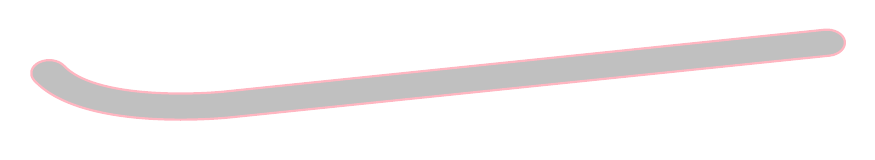
\begin{tikzpicture}
\begin{scope}
[xshift=313pt-0.5cm,yshift=171pt-0.3cm,y=0.80pt, x=0.80pt, yscale=-0.8000000, xscale=-1.1000000, inner sep=0pt, outer sep=0pt,rotate=-20]
      \path[fill=Silver,,draw=LightPink,thick]
        (28.1810,234.4030) .. controls (24.5760,232.5020) and
        (20.1130,233.8830) .. (18.2100,237.4890) .. controls (16.3100,241.0940) and
        (17.6900,245.5590) .. (21.2960,247.4590)
        -- (239.8290,363.9620) .. controls
        (239.9270,364.0140) and (240.1160,364.1190) .. (240.3990,364.2660) .. controls
        (246.5690,367.5190) and (295.5200,392.2130) .. (323.2330,372.3370) .. controls
        (326.5460,369.9620) and (327.3030,365.3510) .. (324.9280,362.0390) .. controls
        (322.5510,358.7260) and (317.9420,357.9690) .. (314.6310,360.3430) .. controls
        (296.8030,373.1290) and (259.6880,357.9110) .. (246.7950,350.9500)
        -- cycle
      ;
    \end{scope}


%\path(current bounding box.north east);
%\pgfgetlastxy{\XCoord}{\YCoord};
%\fill[red,overlay] (current bounding box.north east)circle(2pt)node[above] {\XCoord,\YCoord};
%\path(current bounding box.south west);
%\pgfgetlastxy{\XCoord}{\YCoord};
%\fill[red,overlay] (current bounding box.south west) circle(2pt)node[above] {\XCoord,\YCoord};
\end{tikzpicture}








\end{document}





